\section{Avaliação do Sistema}
   
   A Figura~\ref{fig:prot} mostra os protótipos desenvolvidos para testes iniciais com o sistema (nó final do lado esquerdo e \textit{gateway} do lado direito). Após uma sessão de testes, foi possível avaliar no experimento a eficiência de transmissão e recepção de dados.%, bem como o consumo de energia do nó final.% levando em consideração as possíveis variáveis que impedem a realização de testes.
   
   \begin{figure}[t!]
    \begin{center}
        \centering
        %\setlength{\unitlength}{0.0105in}
        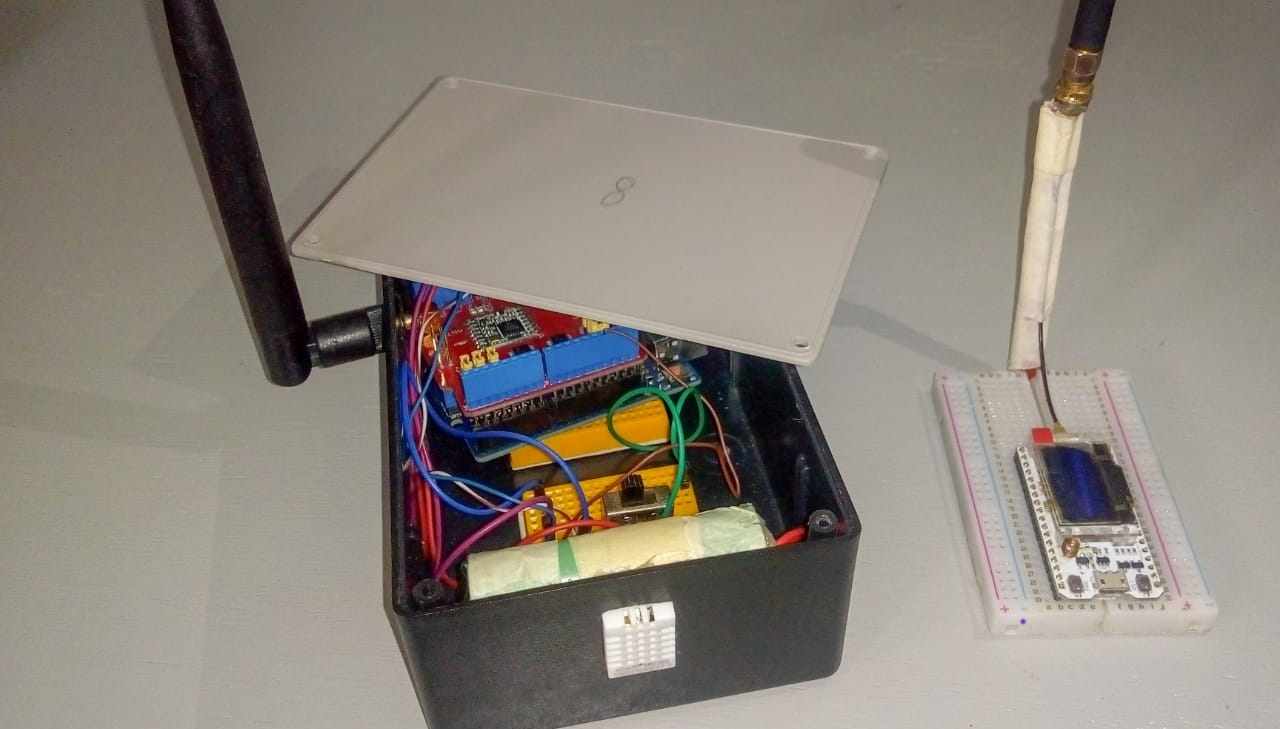
\includegraphics[width=0.4\textwidth]{assets/prototipo.jpeg}
    \end{center}
    \caption{Protótipos desenvolvidos para a realização dos testes.}
    \label{fig:prot}
\end{figure}
   
   Os experimentos foram realizados no bloco dos professores do IFPB--Campus Campina Grande \cite{ref7}. O \textit{gateway} foi posicionado em um espaço, no térreo, enquanto que o transmissor foi posicionado em outro espaço, no sub-solo, distando aproximadamente  60 metros um do outro, e contando com vários obstáculos à comunicação, como paredes densas, laje, objetos metálicos e equipamentos eletrônicos.
   
  O gráfico na Figura~\ref{fig:pdrrssi} apresenta a Taxa de Entrega de Pacote (PDR) a cada hora, em um teste com duração de 24 horas, em que o nó final realizou envios contínuos de pacotes em intervalos de 5 minutos. A PDR geral foi de 78.82\%, no entanto, em alguns momentos a PDR ficou em torno de 20\%, o que pode ter sido ocasionado por modificações no perfil de multi-percurso do ambiente, obstáculos temporários ou presença de fontes de interferência. Considerando a taxa de transmissão de pacote utilizada, com PDR de 20\% ainda é possível obter uma nova informação a cada 25 minutos, em média, o que é suficiente para a realização do monitoramento de temperatura e umidade, que são grandezas que variam lentamente. No entanto, os resultados ressaltam a importância de se desenvolver estratégias para aumento de confiabilidade na transmissão de pacotes de alerta. Pode-se empregar, por exemplo, estratégias de redundância, como replicação de pacote, diversidade de frequência ou de modulação. Essas possibilidades serão estudadas em trabalhos futuros.
   %para permitir um aumento de confiabilidade do sistema.
   
   A Figura~\ref{fig:pdrrssi} também mostra o RSSI médio e o desvio padrão. No protótipo foi utilizado um transceptor  RF96, que pode operar com uma sensibilidade superior a -148dBm [5]. A potência utilizada na transmissão de dados foi  de 17~dBm, que é a potência padrão utilizada na biblioteca do LoRa.%\rd{(precisa saber a sensibilidade do transceptor, para uma discussão melhor. Outra informação importante que faltou foi a potência de transmissão usada.)}
   
    % -------------------- dados legais -------------------- 
    % Potência de transmissão usada:  
    % - +17dBm (a padrão da lib do Arduíno **Lora by Sandeep Mistry** usada)
    % - pode ser configurado +2dBm até +20dBm
   
    % Sensibilidade do transceptor (Tirado do datasheet [3]):
    % - Dynamic Range RSSI -> 127 dB
    % Using Semtech’s patented LoRaTM modulation technique
    % SX1276/77/78/79 can achieve a sensitivity of over -148dBm
    % using a low cost crystal and bill of materials. The high
    % sensitivity combined with the integrated +20 dBm power
    % amplifier yields industry leading link budget making it
    % optimal for any application requiring range or robustness. 
   
   
   \begin{figure}[t!]
        \begin{center}
            \centering
            \setlength{\unitlength}{0.0105in}
            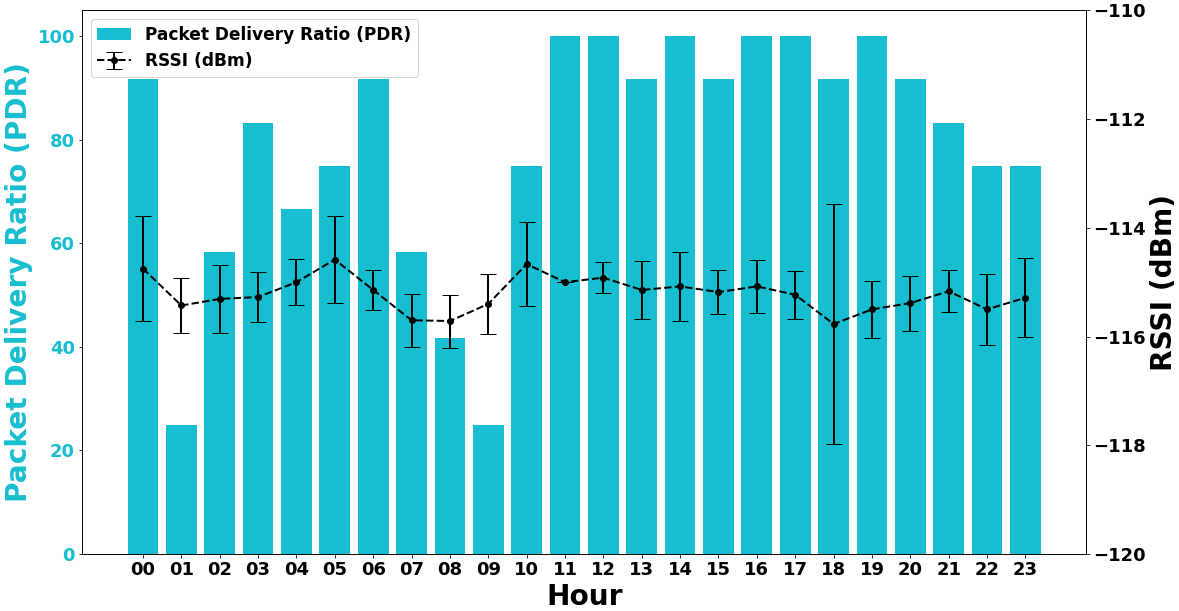
\includegraphics[width=.45\textwidth]{assets/pdr-rssi-5.png}
        \end{center}
        \caption{Percentual em entrega dos pacotes em barras e indicador de intensidade do sinal recebido em linha.}
        \label{fig:pdrrssi}
    \end{figure}